\documentclass{beamer}
\usetheme{Boadilla}
\usecolortheme{seahorse}
\usefonttheme{serif}

\usepackage{lipsum}
\usepackage{graphicx,xcolor}
\usepackage{amsmath,amssymb,amsfonts}
\usepackage{colortbl}

\AtBeginSection[]{ 
    \begin{frame}{Outline} 
        \frametitle{Cuprins}
        \tableofcontents[currentsection] 
    \end{frame} }

\title{Verificarea rețelelor neuronale folosind alpha-beta-CROWN și NeuralSAT pentru benchmark-ul cGan al competiției VNN-Comp2023}

\author{Diaconu Laura \\ Domșa Emanuel \\
Laptedulce Anastasia \\ Morariu Ioana-Alexandra \\
Romaneț Rareș}

\date{}


\titlegraphic{
\includegraphics[width=1.5cm]{images/logo/uvt.jpg}}

\begin{document}

\begin{frame}
\titlepage
\end{frame}


\section{Analiza modului de funcționare a rețelei neuronale}
\begin{frame}{Analiza modului de functionare a retelei neuronale}
    \begin{figure}[ht]
    \centering
    {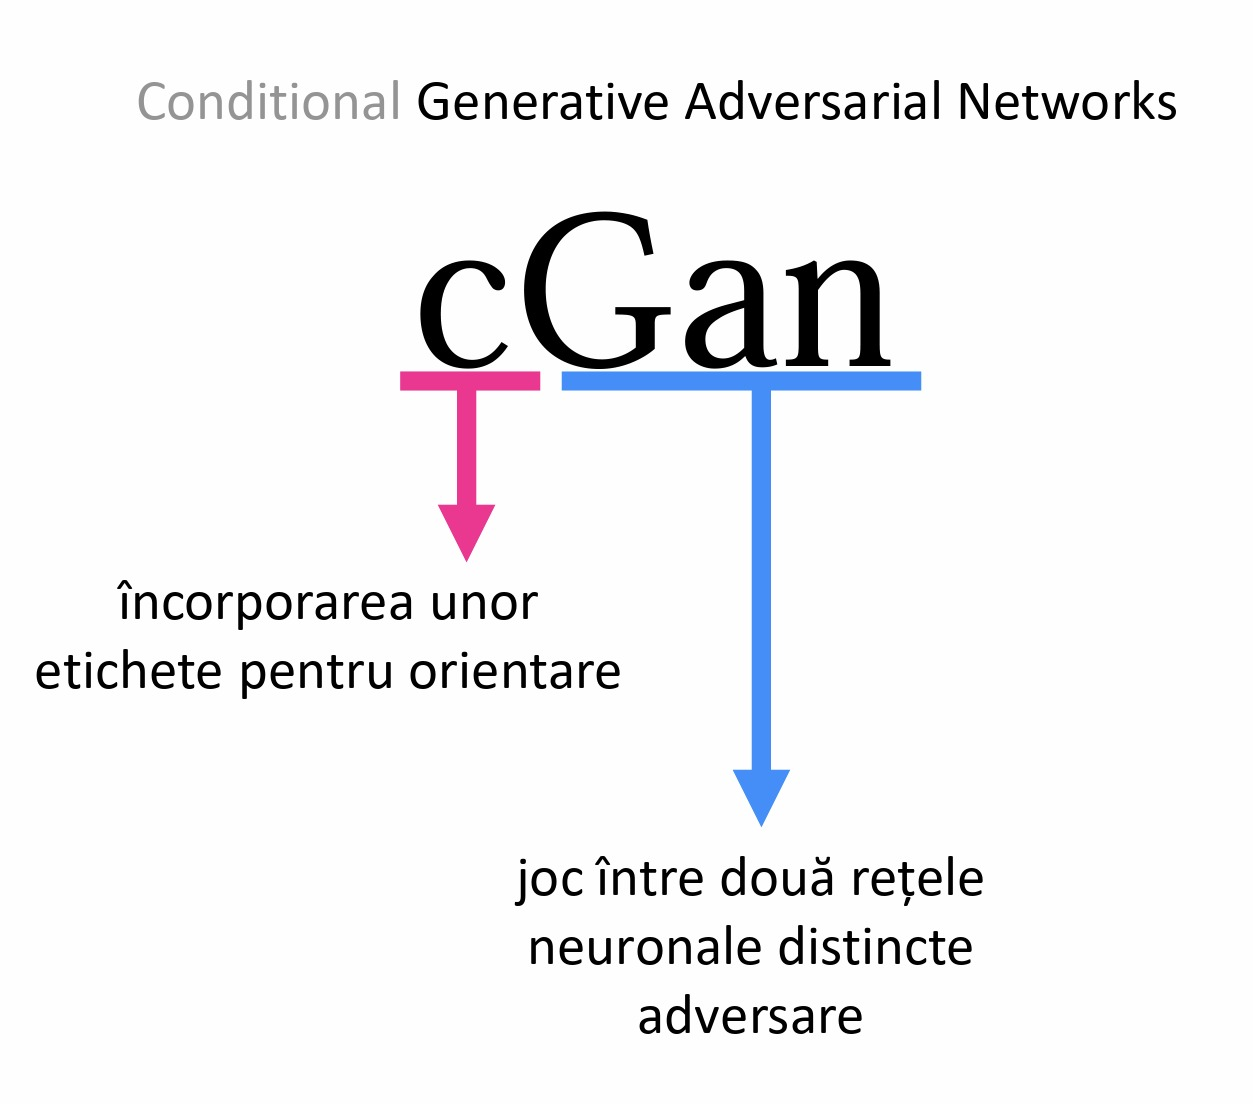
\includegraphics[width=9cm]{images/introducere/Ale_3.jpeg}}
    \label{vnnlib}
    \end{figure}
\end{frame}

\begin{frame}{Analiza modului de functionare a retelei neuronale}
    \begin{figure}[ht]
    \centering
    {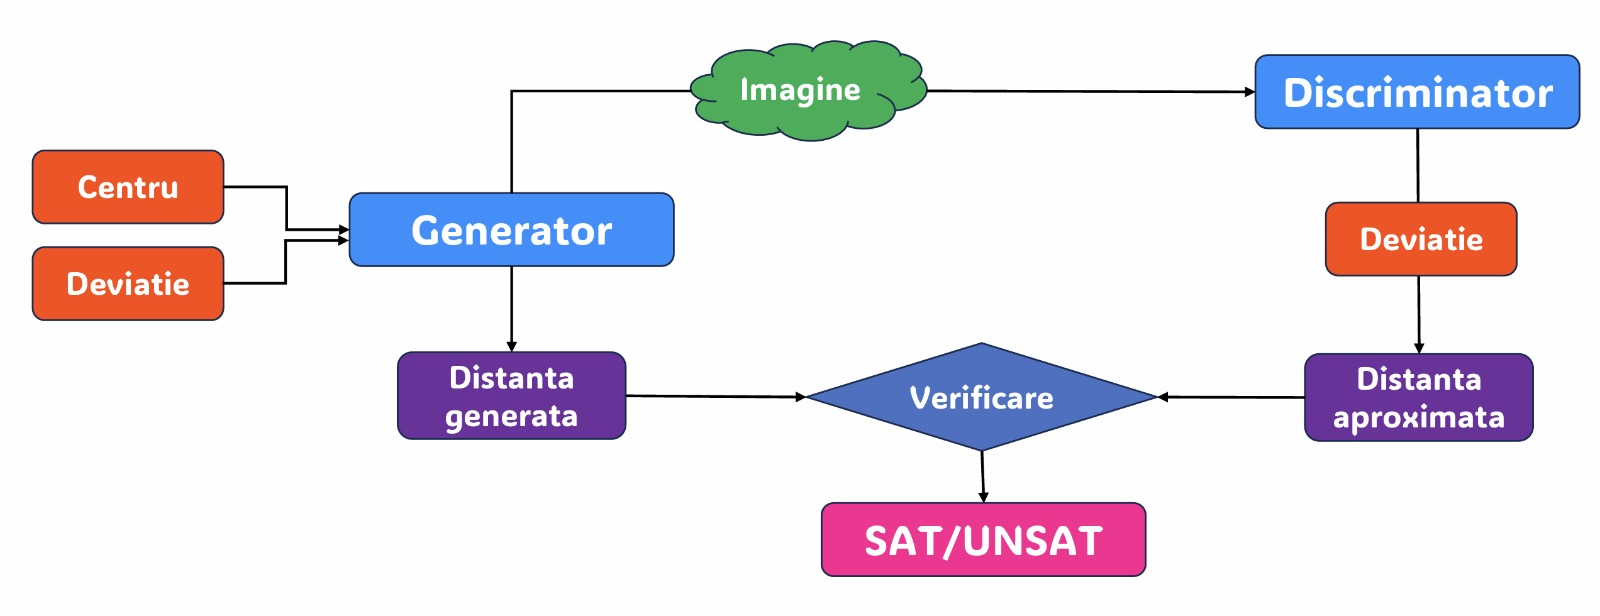
\includegraphics[width=12cm]{images/introducere/Ale_1.jpeg}}
    \label{vnnlib}
    \end{figure}
\end{frame}


\begin{frame}{Analiza modului de functionare a retelei neuronale}   
    \begin{figure}[ht]
    \centering
    {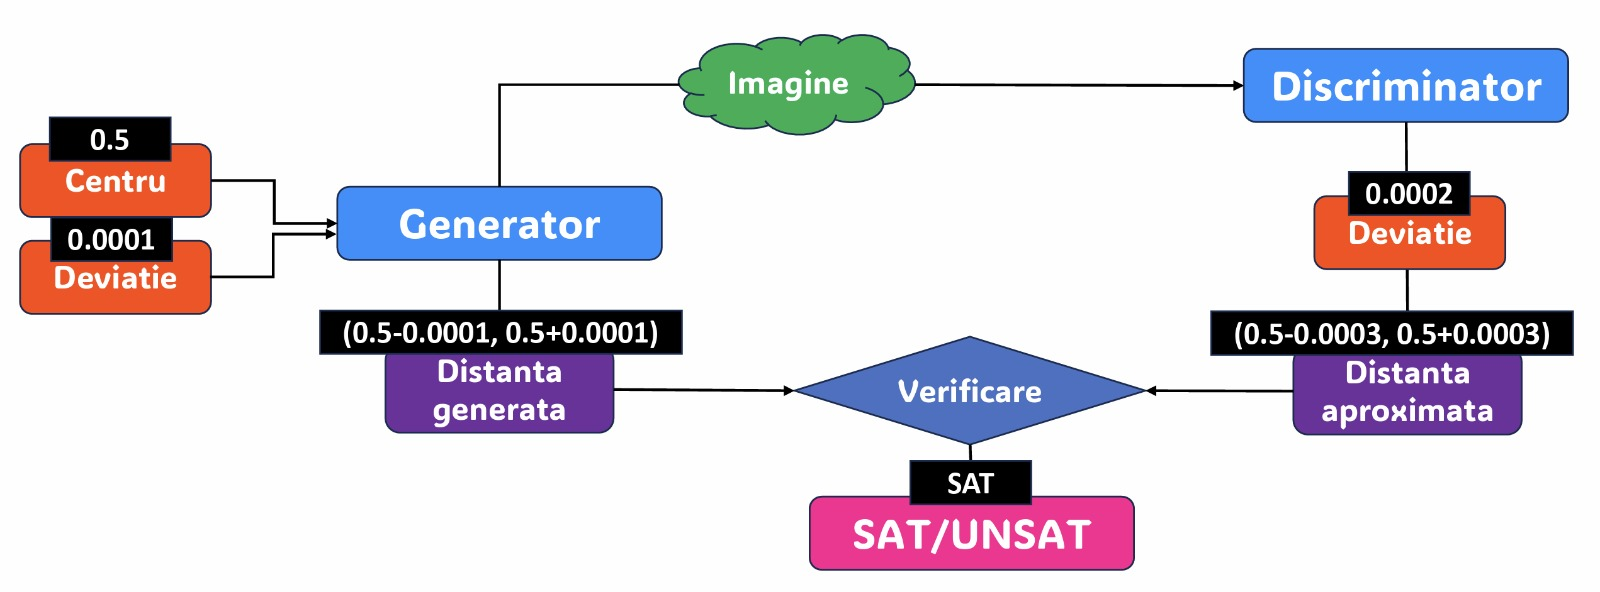
\includegraphics[width=12cm]{images/introducere/Ale_2.jpeg}}
    \label{vnnlib}
    \end{figure}
\end{frame}


\section{Caracterizarea setului de date cGAN}

\begin{frame}{Caracterizarea setului de date}
    \begin{itemize}
        \item verificare corectitudine rețele neuronale
        \item fisiere .onnx
        \item fisiere .vnnlib
        \item denumire sugestivă
    \end{itemize}
\end{frame}

\begin{frame}{Caracterizarea setului de date}
    \begin{figure}[ht]
    \begin{tabular}{cc}
    \hspace{0cm} {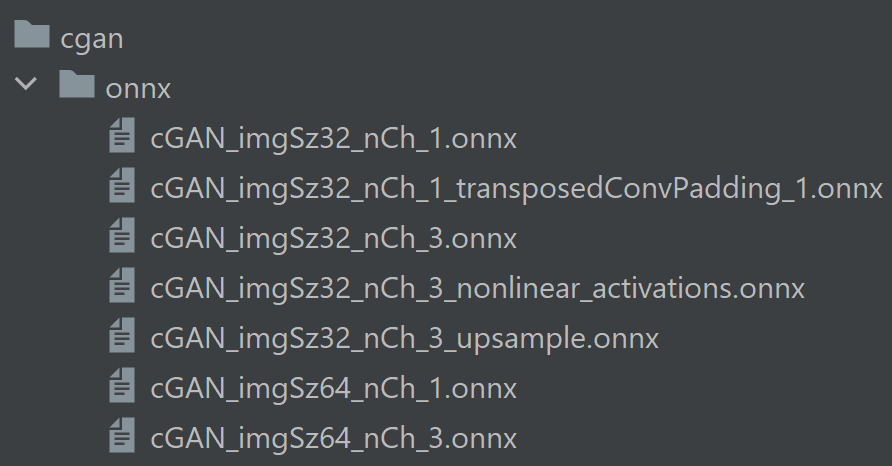
\includegraphics[width=5.5cm]{images/caracterizare/onnx.png}} &
    \hspace{-0.5cm} {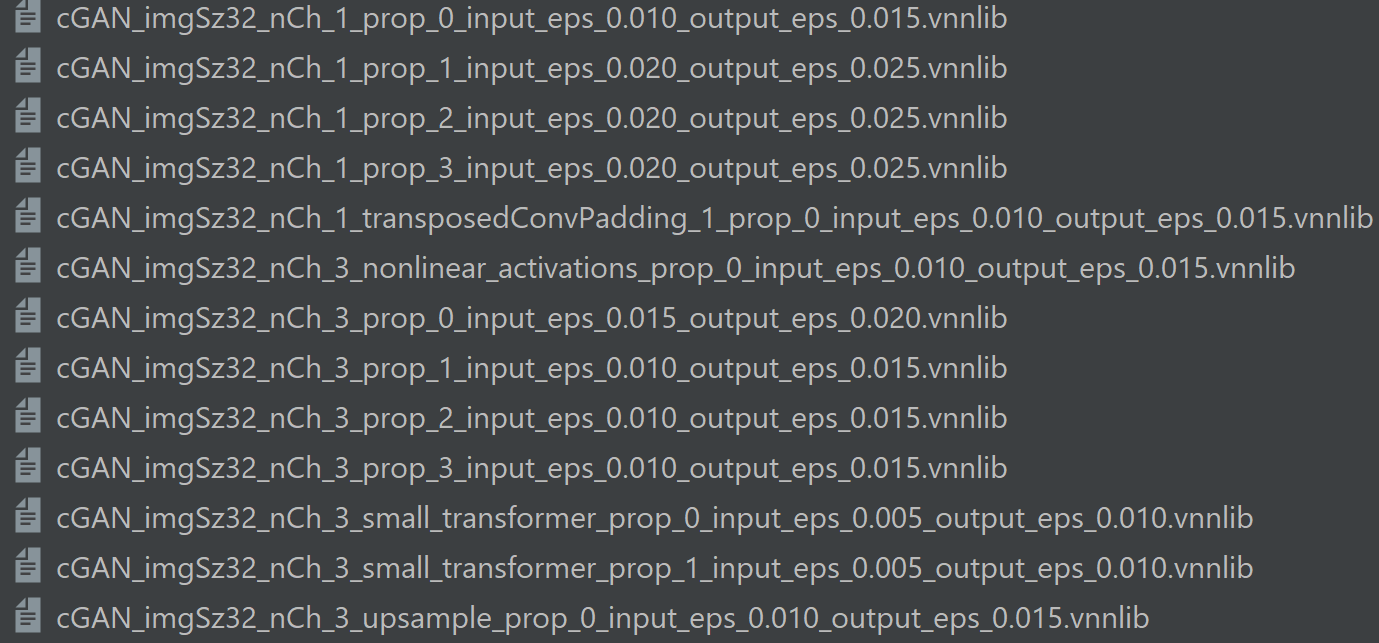
\includegraphics[width=6cm]{images/caracterizare/vnnlib.png}}
    \end{tabular}
    \caption{Fișierele benchmark-ului cGAN}
    \end{figure}
\end{frame}

\begin{frame}{Caracterizarea setului de date}
    \begin{figure}[ht]
    \centering
    {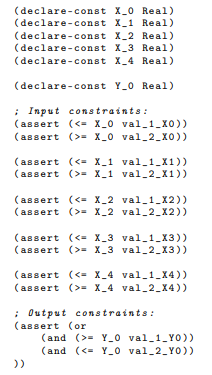
\includegraphics[width=3.5cm]{images/caracterizare/continutVNNLIB.png}}
    \caption{Conținut fișier VNNLIB}
    \label{obstacole}
    \end{figure}
\end{frame}



\section{Configurare tool-uri}
\begin{frame}{Instalare si configurare tool-uri}
    \begin{itemize}
        \item Alpha-beta-CROWN
        \item NeuralSAT
        \item Pași de instalare
        \item Dificultăți întâlnite la instalare
    \end{itemize}
    
    \begin{figure}[ht]
    \centering
    {
\includegraphics[width=10 cm]{images/caracterizare/libcuda.png}}
    \label{obstacole}
    \end{figure}

    \begin{figure}[ht]
    \centering
    {
\includegraphics[width=10 cm]{images/caracterizare/rulareabc.png}}
    \label{obstacole}
    \end{figure}

    \begin{figure}[ht]
    \centering
    {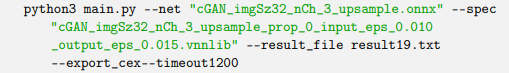
\includegraphics[width=10 cm]{images/caracterizare/rulareneu.png}}
    \label{obstacole}
    \end{figure}
\end{frame}


\section{Interpretare rezultate}
\begin{frame}{Rezultate alpha-beta-CROWN}
    \begin{figure}[ht]
    \centering
    {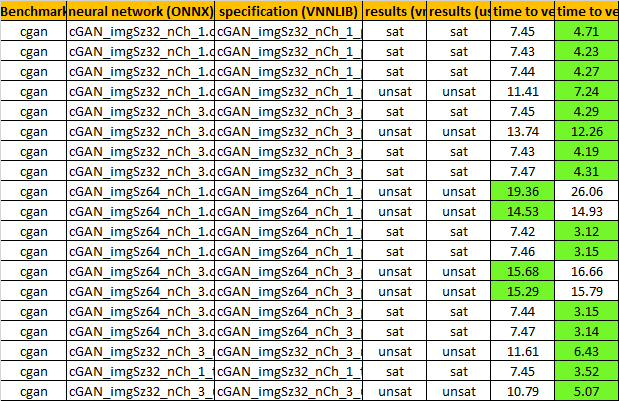
\includegraphics[width=11cm]{images/interpretare/abC_comp_vs_us.png}}
    \label{rezultateAlpha}
    \end{figure}
\end{frame}

\begin{frame}{Rezultate alpha-beta-CROWN}
    \begin{figure}[ht]
    \centering
    {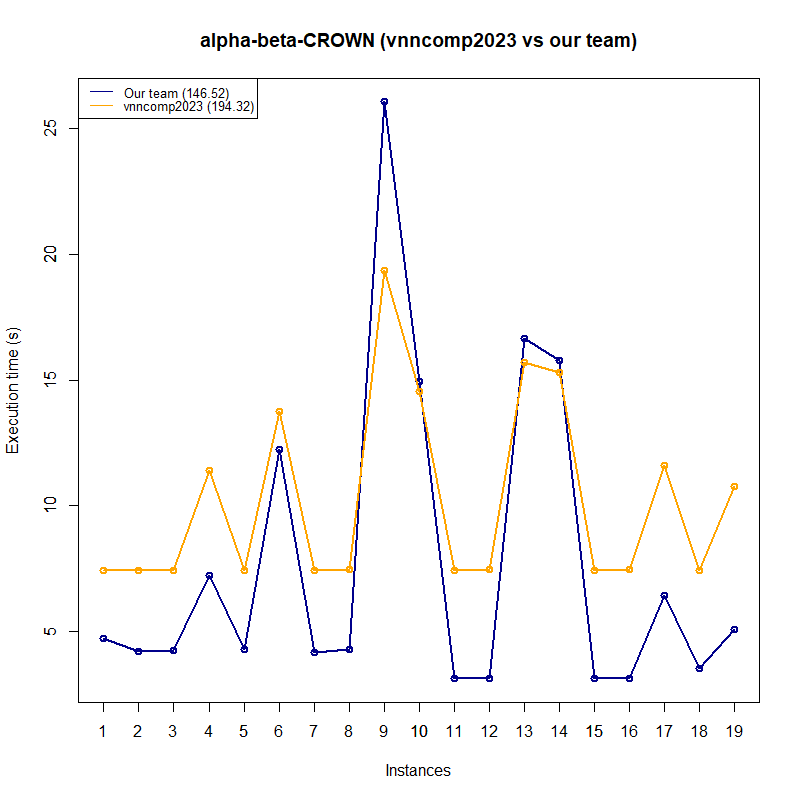
\includegraphics[width=8cm]{images/interpretare/abC_us_vs_vnncomp.png}}
    \label{rezultateAlpha}
    \end{figure}
\end{frame}

\begin{frame}{Rezultate NeuralSAT}
    \begin{figure}[ht]
    \centering
    {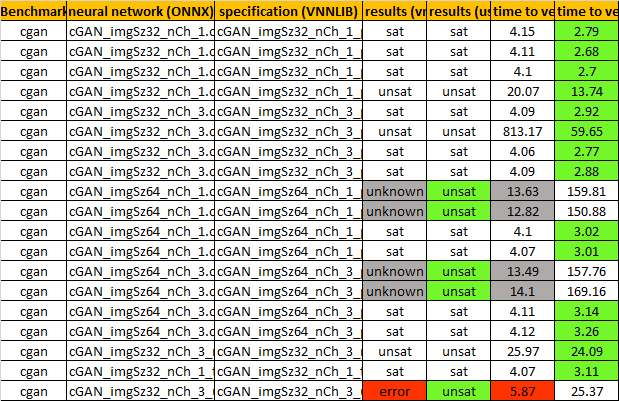
\includegraphics[width=11cm]{images/interpretare/NeuralSAT_comp_vs_us.png}}
    \label{rezultateNeuralSat}
    \end{figure}
\end{frame}

\begin{frame}{Rezultate NeuralSAT}
    \begin{figure}[ht]
    \centering
    {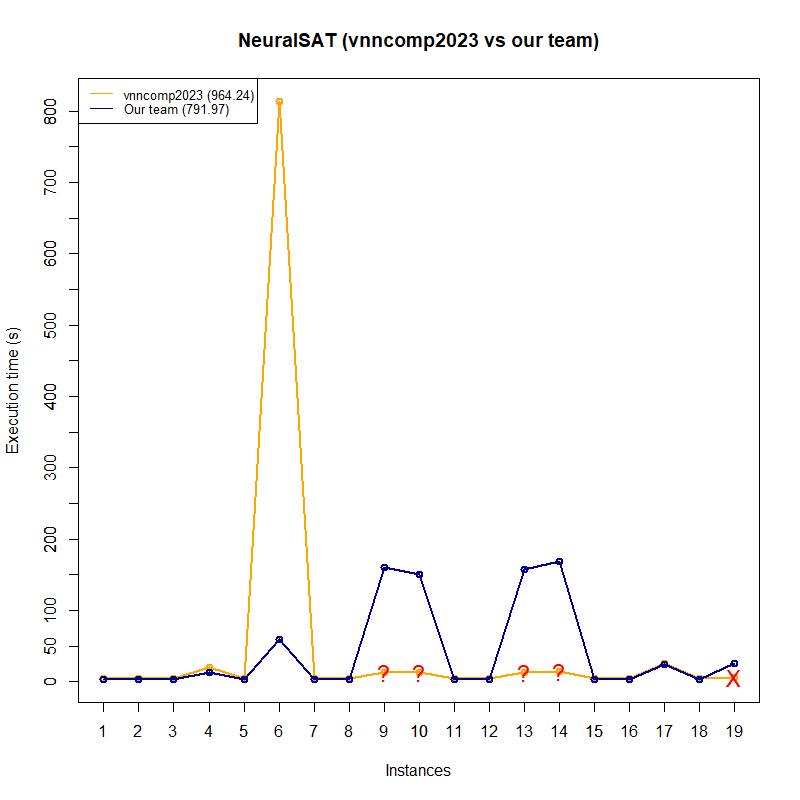
\includegraphics[width=8cm]{images/interpretare/NeuralSAT_us_vs_vnncomp2023.png}}
    \label{rezultateNeuralSat}
    \end{figure}
\end{frame}

\begin{frame}{Rezultate alpha-beta-CROWN vs NeuralSAT}
    \begin{figure}[ht]
    \centering
    {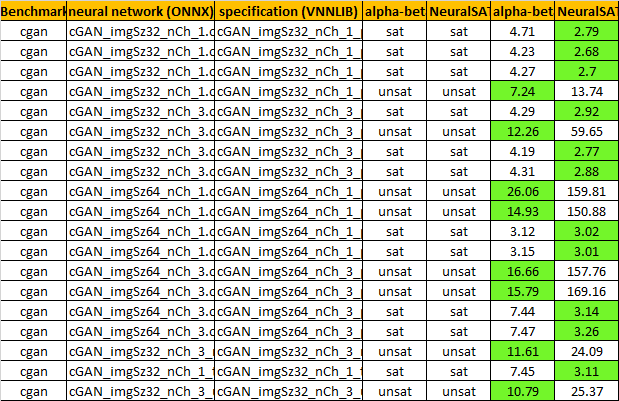
\includegraphics[width=11cm]{images/interpretare/alpha-beta-CROWN_vs_NeuralSAT.png}}
    \label{rezultateNeuralSat}
    \end{figure}
\end{frame}

\begin{frame}{Rezultate alpha-beta-CROWN vs NeuralSAT}
    \begin{figure}[ht]
    \centering
    {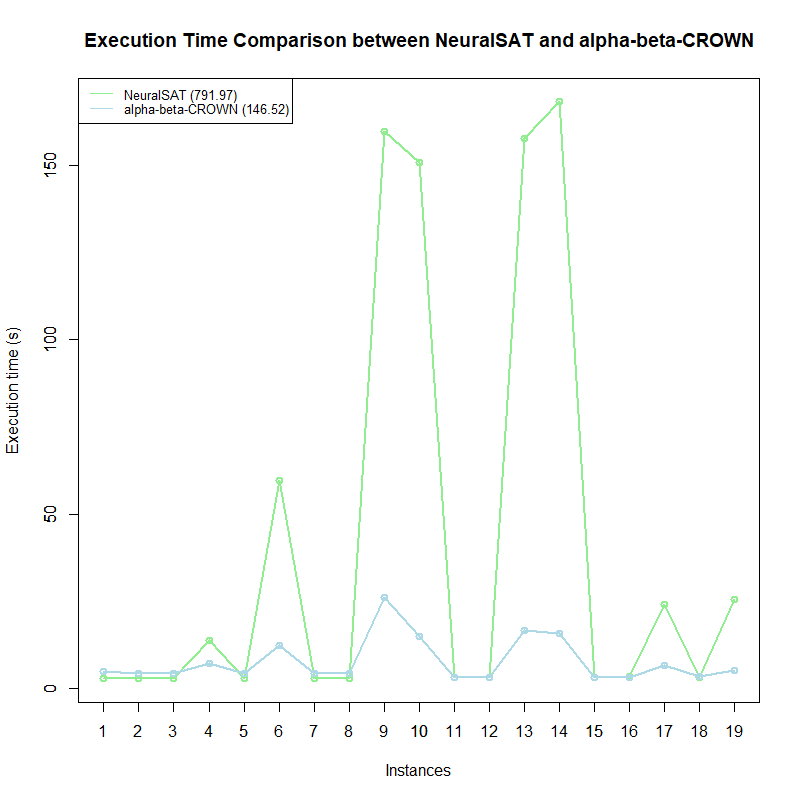
\includegraphics[width=8cm]{images/interpretare/Exec_time_comparison.png}}
    \label{rezultateNeuralSat}
    \end{figure}
\end{frame}

\begin{frame}{Rezultate alpha-beta-CROWN vs NeuralSAT}
    \begin{figure}[ht]
    \centering
    {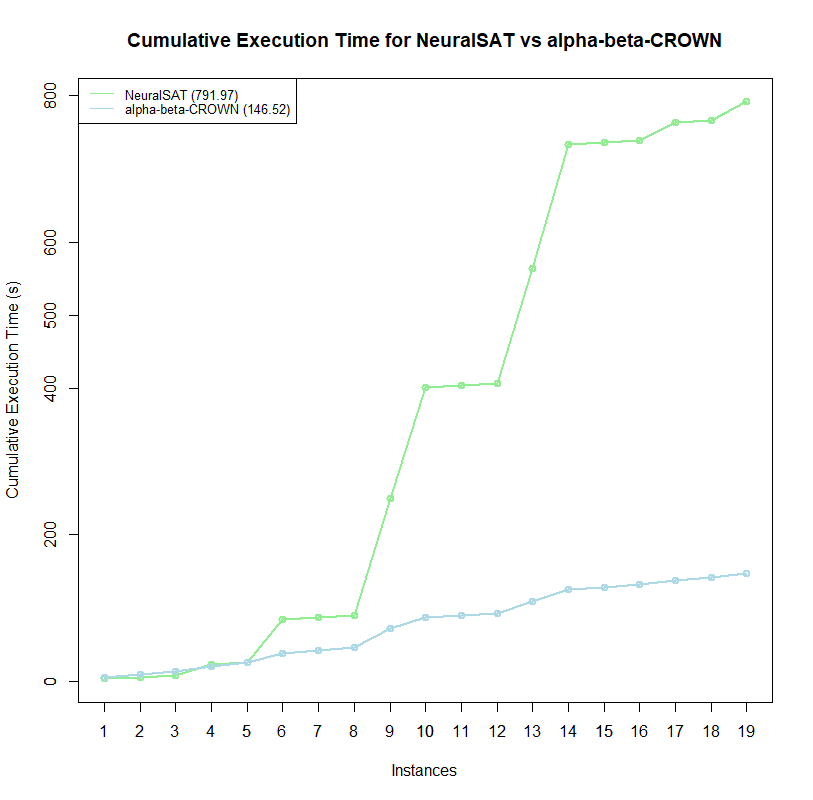
\includegraphics[width=8cm]{images/interpretare/cumulative_NeuralSAT_vs_abC.png}}
    \label{rezultateNeuralSat}
    \end{figure}
\end{frame}

\begin{frame}{Rezultate}
    \begin{figure}[ht]
    \centering
    {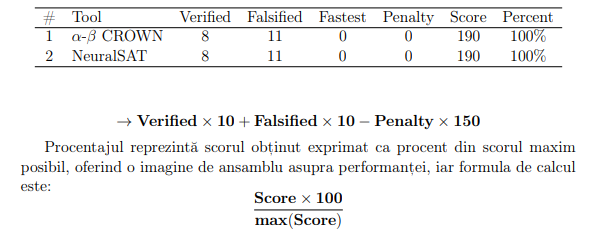
\includegraphics[width=10cm]{images/interpretare/formula.png}}
    \label{tabelTotal}
    \end{figure}
\end{frame}







































% \begin{frame}{Rezultate obtinute folosind alpha\textunderscore beta\textunderscore crown}   
%     \begin{table}[H]
%     \centering
%     \begin{adjustwidth}{}{} % Specifică cât de mult să depășească în stânga și în dreapta
%     \setlength{\tabcolsep}{0pt} % Ajustează spațiul între coloane
%     \renewcommand{\arraystretch}{1.7} % Ajustează spațiul între rânduri
%     \resizebox{\textwidth}{!}{%
%     \begin{tabular}{|c|c|c|c|c|}
%     \hline
%       \textbf{ONNX} & \textbf{VNNLIB} & \textbf{Result} & \textbf{Time to verify (s) } \\
%       \hline
%       cGAN\_imgSz32\_nCh\_1. & cGAN\_imgSz32\_nCh\_1\_prop\_0\_input\_eps\_0.010\_output\_eps\_0.015. & sat & 4.39915 \\
%       cGAN\_imgSz32\_nCh\_1. & cGAN\_imgSz32\_nCh\_1\_prop\_1\_input\_eps\_0.020\_output\_eps\_0.025. & sat & 4.45147 \\
%       cGAN\_imgSz32\_nCh\_1. & cGAN\_imgSz32\_nCh\_1\_prop\_2\_input\_eps\_0.020\_output\_eps\_0.025. & sat & 4.37929  \\
%       cGAN\_imgSz32\_nCh\_1. & cGAN\_imgSz32\_nCh\_1\_prop\_3\_input\_eps\_0.020\_output\_eps\_0.025. &  \cellcolor{gray} unsat & 11.11230  \\
%       cGAN\_imgSz32\_nCh\_3. & cGAN\_imgSz32\_nCh\_3\_prop\_0\_input\_eps\_0.015\_output\_eps\_0.020. & sat & 4.42455 \\
%       cGAN\_imgSz32\_nCh\_3. & cGAN\_imgSz32\_nCh\_3\_prop\_1\_input\_eps\_0.010\_output\_eps\_0.015. & \cellcolor{gray} unsat & 16.71046  \\
%       cGAN\_imgSz32\_nCh\_3. & cGAN\_imgSz32\_nCh\_3\_prop\_2\_input\_eps\_0.010\_output\_eps\_0.015. & sat & 4.31144 \\
%       cGAN\_imgSz32\_nCh\_3. & cGAN\_imgSz32\_nCh\_3\_prop\_3\_input\_eps\_0.010\_output\_eps\_0.015. & sat & 4.40774 \\
%       cGAN\_imgSz64\_nCh\_1. & cGAN\_imgSz64\_nCh\_1\_prop\_0\_input\_eps\_0.010\_output\_eps\_0.015. & \cellcolor{gray} unsat & 30.27740  \\
%       cGAN\_imgSz64\_nCh\_1. & cGAN\_imgSz64\_nCh\_1\_prop\_1\_input\_eps\_0.005\_output\_eps\_0.010. & \cellcolor{gray} unsat & 19.29929  \\
%       cGAN\_imgSz64\_nCh\_1. & cGAN\_imgSz64\_nCh\_1\_prop\_2\_input\_eps\_0.010\_output\_eps\_0.015. & sat & 4.42568  \\
%       cGAN\_imgSz64\_nCh\_1. & cGAN\_imgSz64\_nCh\_1\_prop\_3\_input\_eps\_0.005\_output\_eps\_0.010. & sat & 4.42309  \\
%       cGAN\_imgSz64\_nCh\_3. & cGAN\_imgSz64\_nCh\_3\_prop\_0\_input\_eps\_0.010\_output\_eps\_0.015. & \cellcolor{gray} unsat & 21.70824  \\
%       cGAN\_imgSz64\_nCh\_3. & cGAN\_imgSz64\_nCh\_3\_prop\_1\_input\_eps\_0.010\_output\_eps\_0.015. & \cellcolor{gray} unsat & 21.05809  \\
%       cGAN\_imgSz64\_nCh\_3. & cGAN\_imgSz64\_nCh\_3\_prop\_2\_input\_eps\_0.005\_output\_eps\_0.010. & sat & 4.37459  \\
%       cGAN\_imgSz64\_nCh\_3. & cGAN\_imgSz64\_nCh\_3\_prop\_3\_input\_eps\_0.010\_output\_eps\_0.015. & sat & 4.47376  \\
%       cGAN\_imgSz32\_nCh\_3\_nonlinear\_activations. & cGAN\_imgSz32\_nCh\_3\_nonlinear\_activations\_prop\_0\_input\_eps\_0.010\_output\_eps\_0.015. & \cellcolor{gray} unsat & 10.39218  \\
%       cGAN\_imgSz32\_nCh\_1\_transposedConvPadding\_1. & cGAN\_imgSz32\_nCh\_1\_transposedConvPadding\_1\_prop\_0\_input\_eps\_0.010\_output\_eps\_0.015. & sat & 4.41804  \\
%       cGAN\_imgSz32\_nCh\_3\_upsample. & cGAN\_imgSz32\_nCh\_3\_upsample\_prop\_0\_input\_eps\_0.010\_output\_eps\_0.015. & \cellcolor{gray} unsat & 9.82781  \\
%       \hline
%     \end{tabular}%
%     }
%   \end{adjustwidth}
%   \end{table}
% \end{frame}

% \begin{frame}{Rezultate obtinute in competitie folosind alpha\textunderscore beta\textunderscore crown}   
% \begin{table}[htbp]
%   \centering
%   \setlength{\tabcolsep}{0pt} % Ajustează spațiul între coloane
%   \renewcommand{\arraystretch}{1.7} % Ajustează spațiul între rânduri
%   \resizebox{\textwidth}{!}{%
%     \begin{tabular}{|c|c|c|c|c|c|}
%       \hline
%       \textbf{Benchmark} & \textbf{Neural Network (ONNX)} & \textbf{Specification (VNNLIB)} & \textbf{Result} & \textbf{Time to Verify (s)} \\
%       \hline
%       cgan & cGAN\_imgSz32\_nCh\_1. & cGAN\_imgSz32\_nCh\_1\_prop\_0\_input\_eps\_0.010\_output\_eps\_0.015.  & sat & 7.45 \\
%       cgan & cGAN\_imgSz32\_nCh\_1. & cGAN\_imgSz32\_nCh\_1\_prop\_1\_input\_eps\_0.020\_output\_eps\_0.025.  & sat & 7.43 \\
%       cgan & cGAN\_imgSz32\_nCh\_1. & cGAN\_imgSz32\_nCh\_1\_prop\_2\_input\_eps\_0.020\_output\_eps\_0.025.  & sat & 7.44 \\
%       cgan & cGAN\_imgSz32\_nCh\_1. & cGAN\_imgSz32\_nCh\_1\_prop\_3\_input\_eps\_0.020\_output\_eps\_0.025.  & \cellcolor{gray}unsat & 11.41 \\
%       cgan & cGAN\_imgSz32\_nCh\_3. & cGAN\_imgSz32\_nCh\_3\_prop\_0\_input\_eps\_0.015\_output\_eps\_0.020.  & sat & 7.45 \\
%       cgan & cGAN\_imgSz32\_nCh\_3. & cGAN\_imgSz32\_nCh\_3\_prop\_1\_input\_eps\_0.010\_output\_eps\_0.015.  & \cellcolor{gray}unsat & 13.74 \\
%       cgan & cGAN\_imgSz32\_nCh\_3. & cGAN\_imgSz32\_nCh\_3\_prop\_2\_input\_eps\_0.010\_output\_eps\_0.015.  & sat & 7.43 \\
%       cgan & cGAN\_imgSz32\_nCh\_3. & cGAN\_imgSz32\_nCh\_3\_prop\_3\_input\_eps\_0.010\_output\_eps\_0.015.  & sat & 7.47 \\
%       cgan & cGAN\_imgSz64\_nCh\_1. & cGAN\_imgSz64\_nCh\_1\_prop\_0\_input\_eps\_0.010\_output\_eps\_0.015.  & \cellcolor{gray}unsat & 19.36 \\
%       cgan & cGAN\_imgSz64\_nCh\_1. & cGAN\_imgSz64\_nCh\_1\_prop\_1\_input\_eps\_0.005\_output\_eps\_0.010.  & \cellcolor{gray}unsat & 14.53 \\
%       cgan & cGAN\_imgSz64\_nCh\_1. & cGAN\_imgSz64\_nCh\_1\_prop\_2\_input\_eps\_0.010\_output\_eps\_0.015.  & sat & 7.42 \\
%       cgan & cGAN\_imgSz64\_nCh\_1. & cGAN\_imgSz64\_nCh\_1\_prop\_3\_input\_eps\_0.005\_output\_eps\_0.010.  & sat & 7.46 \\
%       cgan & cGAN\_imgSz64\_nCh\_3. & cGAN\_imgSz64\_nCh\_3\_prop\_0\_input\_eps\_0.010\_output\_eps\_0.015.  & \cellcolor{gray}unsat & 15.68 \\
%       cgan & cGAN\_imgSz64\_nCh\_3. & cGAN\_imgSz64\_nCh\_3\_prop\_1\_input\_eps\_0.010\_output\_eps\_0.015.  & \cellcolor{gray}unsat & 15.29 \\
%       cgan & cGAN\_imgSz64\_nCh\_3. & cGAN\_imgSz64\_nCh\_3\_prop\_2\_input\_eps\_0.005\_output\_eps\_0.010.  & sat & 7.44 \\
%       cgan & cGAN\_imgSz64\_nCh\_3. & cGAN\_imgSz64\_nCh\_3\_prop\_3\_input\_eps\_0.010\_output\_eps\_0.015.  & sat & 7.47 \\
%       cgan & cGAN\_imgSz32\_nCh\_3\_nonlinear\_activations. & cGAN\_imgSz32\_nCh\_3\_nonlinear\_activations\_prop\_0\_input\_eps\_0.010\_output\_eps\_0.015. & \cellcolor{gray}unsat & 11.61 \\
%       cgan & cGAN\_imgSz32\_nCh\_1\_transposedConvPadding\_1. & cGAN\_imgSz32\_nCh\_1\_transposedConvPadding\_1\_prop\_0\_input\_eps\_0.010\_output\_eps\_0.015. & sat & 7.45 \\
%       cgan & cGAN\_imgSz32\_nCh\_3\_upsample. & cGAN\_imgSz32\_nCh\_3\_upsample\_prop\_0\_input\_eps\_0.010\_output\_eps\_0.015. & \cellcolor{gray}unsat & 10.79 \\
%       \hline
%     \end{tabular}%
%     }
%     \end{table}
% \end{frame}

% \begin{frame}{Rezultate obtinute folosind NeuralSat}   
% \begin{table}[H]
%   \centering
%   \begin{adjustwidth}{}{} % Specifică cât de mult să depășească în stânga și în dreapta
%   \setlength{\tabcolsep}{0pt} % Ajustează spațiul între coloane
%   \renewcommand{\arraystretch}{1.7} % Ajustează spațiul între rânduri
%   \resizebox{\textwidth}{!}{%
%     \begin{tabular}{|c|c|c|c|c|}
%       \hline
%       \textbf{Benchmark} & \textbf{ONNX} & \textbf{Specification (VNNLIB)} & \textbf{Result} & \textbf{Time to Verify (s)} \\
%       \hline
%       cgan & cGAN\_imgSz32\_nCh\_1. & cGAN\_imgSz32\_nCh\_1\_prop\_0\_input\_eps\_0.010\_output\_eps\_0.015. & sat & 3.175035 \\
%       cgan & cGAN\_imgSz32\_nCh\_1. & cGAN\_imgSz32\_nCh\_1\_prop\_1\_input\_eps\_0.020\_output\_eps\_0.025. & sat & 3.137382 \\
%       cgan & cGAN\_imgSz32\_nCh\_1. & cGAN\_imgSz32\_nCh\_1\_prop\_2\_input\_eps\_0.020\_output\_eps\_0.025. & sat & 3.126519 \\
%       cgan & cGAN\_imgSz32\_nCh\_1. & cGAN\_imgSz32\_nCh\_1\_prop\_3\_input\_eps\_0.020\_output\_eps\_0.025. & \cellcolor{gray}unsat & 13.556497 \\
%       cgan & cGAN\_imgSz32\_nCh\_3. & cGAN\_imgSz32\_nCh\_3\_prop\_0\_input\_eps\_0.015\_output\_eps\_0.020. & sat & 4.432113 \\
%       cgan & cGAN\_imgSz32\_nCh\_3. & cGAN\_imgSz32\_nCh\_3\_prop\_1\_input\_eps\_0.010\_output\_eps\_0.015. & \cellcolor{gray}unsat & 60.970006 \\
%       cgan & cGAN\_imgSz32\_nCh\_3. & cGAN\_imgSz32\_nCh\_3\_prop\_2\_input\_eps\_0.010\_output\_eps\_0.015. & sat & 3.205494 \\
%       cgan & cGAN\_imgSz32\_nCh\_3. & cGAN\_imgSz32\_nCh\_3\_prop\_3\_input\_eps\_0.010\_output\_eps\_0.015. & sat & 3.269871 \\
%       cgan & cGAN\_imgSz64\_nCh\_1. & cGAN\_imgSz64\_nCh\_1\_prop\_0\_input\_eps\_0.010\_output\_eps\_0.015. & \cellcolor{gray}unsat & 161.189276 \\
%       cgan & cGAN\_imgSz64\_nCh\_1. & cGAN\_imgSz64\_nCh\_1\_prop\_1\_input\_eps\_0.005\_output\_eps\_0.010. & \cellcolor{gray}unsat & 173.990763 \\
%       cgan & cGAN\_imgSz64\_nCh\_1. & cGAN\_imgSz64\_nCh\_1\_prop\_2\_input\_eps\_0.010\_output\_eps\_0.015. & sat & 4.552644 \\
%       cgan & cGAN\_imgSz64\_nCh\_1. & cGAN\_imgSz64\_nCh\_1\_prop\_3\_input\_eps\_0.005\_output\_eps\_0.010. & sat & 3.337892 \\
%       cgan & cGAN\_imgSz64\_nCh\_3. & cGAN\_imgSz64\_nCh\_3\_prop\_0\_input\_eps\_0.010\_output\_eps\_0.015. & \cellcolor{gray}unsat & 159.679505 \\
%       cgan & cGAN\_imgSz64\_nCh\_3. & cGAN\_imgSz64\_nCh\_3\_prop\_1\_input\_eps\_0.010\_output\_eps\_0.015. & \cellcolor{gray}unsat & 175.243838 \\
%       cgan & cGAN\_imgSz64\_nCh\_3. & cGAN\_imgSz64\_nCh\_3\_prop\_2\_input\_eps\_0.005\_output\_eps\_0.010. & sat & 3.311298 \\
%       cgan & cGAN\_imgSz64\_nCh\_3. & cGAN\_imgSz64\_nCh\_3\_prop\_3\_input\_eps\_0.010\_output\_eps\_0.015. & sat & 4.474263 \\
%       cgan & cGAN\_imgSz32\_nCh\_3\_nonlinear\_activations. & cGAN\_imgSz32\_nCh\_3\_nonlinear\_activations\_prop\_0\_input\_eps\_0.010\_output\_eps\_0.015. & \cellcolor{gray}unsat & 22.691869 \\
%       cgan & cGAN\_imgSz32\_nCh\_1\_transposedConvPadding\_1. & cGAN\_imgSz32\_nCh\_1\_transposedConvPadding\_1\_prop\_0\_input\_eps\_0.010\_output\_eps\_0.015. & sat & 3.235317 \\
%       cgan & cGAN\_imgSz32\_nCh\_3\_upsample. & cGAN\_imgSz32\_nCh\_3\_upsample\_prop\_0\_input\_eps\_0.010\_output\_eps\_0.015. & \cellcolor{gray}unsat & 24.717013 \\
%       \hline
%     \end{tabular}%
%   }
%   \end{adjustwidth}
% \end{table}
% \end{frame}

% \begin{frame}{Rezultate obtinute in competitie folosind NeuralSat}   
% \begin{table}[htbp]
%   \centering
%   \setlength{\tabcolsep}{0pt} % Ajustează spațiul între coloane
%   \renewcommand{\arraystretch}{1.7} % Ajustează spațiul între rânduri
%   \resizebox{\textwidth}{!}{%
%     \begin{tabular}{|c|c|c|c|c|c|}
%       \hline
%       \textbf{Benchmark} & \textbf{Neural Network (ONNX)} & \textbf{Specification (VNNLIB)}  & \textbf{Result} & \textbf{Time to Verify (s)} \\
%       \hline
%       cgan & cGAN\_imgSz32\_nCh\_1. & cGAN\_imgSz32\_nCh\_1\_prop\_0\_input\_eps\_0.010\_output\_eps\_0.015.  & sat & 4.158000 \\
%       cgan & cGAN\_imgSz32\_nCh\_1. & cGAN\_imgSz32\_nCh\_1\_prop\_1\_input\_eps\_0.020\_output\_eps\_0.025.  & sat & 4.106945 \\
%       cgan & cGAN\_imgSz32\_nCh\_1. & cGAN\_imgSz32\_nCh\_1\_prop\_2\_input\_eps\_0.020\_output\_eps\_0.025.  & sat & 4.100790\\
%       cgan & cGAN\_imgSz32\_nCh\_1. & cGAN\_imgSz32\_nCh\_1\_prop\_3\_input\_eps\_0.020\_output\_eps\_0.025.  & \cellcolor{gray}unsat & 20.074181 \\
%       cgan & cGAN\_imgSz32\_nCh\_3. & cGAN\_imgSz32\_nCh\_3\_prop\_0\_input\_eps\_0.015\_output\_eps\_0.020.  & sat & 4.090721 \\
%       cgan & cGAN\_imgSz32\_nCh\_3. & cGAN\_imgSz32\_nCh\_3\_prop\_1\_input\_eps\_0.010\_output\_eps\_0.015.  & \cellcolor{gray}unsat & 813.175559 \\
%       cgan & cGAN\_imgSz32\_nCh\_3. & cGAN\_imgSz32\_nCh\_3\_prop\_2\_input\_eps\_0.010\_output\_eps\_0.015.  & sat & 4.062533 \\
%       cgan & cGAN\_imgSz32\_nCh\_3. & cGAN\_imgSz32\_nCh\_3\_prop\_3\_input\_eps\_0.010\_output\_eps\_0.015.  & sat & 4.093121 \\
%       cgan & cGAN\_imgSz64\_nCh\_1. & cGAN\_imgSz64\_nCh\_1\_prop\_0\_input\_eps\_0.010\_output\_eps\_0.015.  & \cellcolor{red}unknown & 13.634478 \\
%       cgan & cGAN\_imgSz64\_nCh\_1. & cGAN\_imgSz64\_nCh\_1\_prop\_1\_input\_eps\_0.005\_output\_eps\_0.010.  & \cellcolor{red}unknown & 12.826754 \\
%       cgan & cGAN\_imgSz64\_nCh\_1. & cGAN\_imgSz64\_nCh\_1\_prop\_2\_input\_eps\_0.010\_output\_eps\_0.015.  & sat & 4.101576 \\
%       cgan & cGAN\_imgSz64\_nCh\_1. & cGAN\_imgSz64\_nCh\_1\_prop\_3\_input\_eps\_0.005\_output\_eps\_0.010.  & sat & 4.076540\\
%       cgan & cGAN\_imgSz64\_nCh\_3. & cGAN\_imgSz64\_nCh\_3\_prop\_0\_input\_eps\_0.010\_output\_eps\_0.015.  & \cellcolor{red}unknown & 13.494352 \\
%       cgan & cGAN\_imgSz64\_nCh\_3. & cGAN\_imgSz64\_nCh\_3\_prop\_1\_input\_eps\_0.010\_output\_eps\_0.015.  & \cellcolor{red}unknown & 14.104266 \\
%       cgan & cGAN\_imgSz64\_nCh\_3. & cGAN\_imgSz64\_nCh\_3\_prop\_2\_input\_eps\_0.005\_output\_eps\_0.010.  & sat & 4.106288 \\
%       cgan & cGAN\_imgSz64\_nCh\_3. & cGAN\_imgSz64\_nCh\_3\_prop\_3\_input\_eps\_0.010\_output\_eps\_0.015.  & sat & 4.119278 \\
%       cgan & cGAN\_imgSz32\_nCh\_3\_nonlinear\_activations. & cGAN\_imgSz32\_nCh\_3\_nonlinear\_activations\_prop\_0\_input\_eps\_0.010\_output\_eps\_0.015.  & \cellcolor{gray}unsat & 25.971333 \\
%       cgan & cGAN\_imgSz32\_nCh\_1\_transposedConvPadding\_1. & cGAN\_imgSz32\_nCh\_1\_transposedConvPadding\_1\_prop\_0\_input\_eps\_0.010\_output\_eps\_0.015.  & sat & 4.069863 \\
%       cgan & cGAN\_imgSz32\_nCh\_3\_upsample. & cGAN\_imgSz32\_nCh\_3\_upsample\_prop\_0\_input\_eps\_0.010\_output\_eps\_0.015.  & \cellcolor{red}error & 5.869110 \\
%       \hline
%     \end{tabular}%
%   }
% \end{table}
% \end{frame}






\section{Rețele neuronale în simularea provocărilor reale}
\begin{frame}{Rețele neuronale în simularea provocarilor reale}   
    \begin{figure}[ht]
    \centering
    {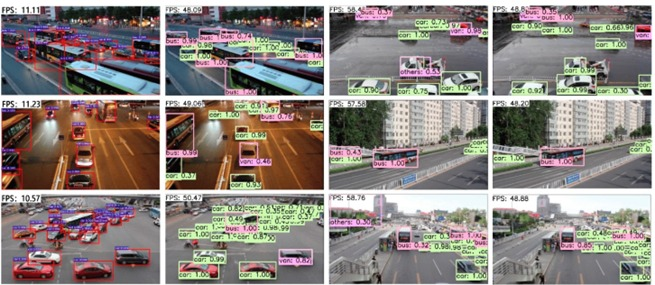
\includegraphics[width=12cm]{images/aplicatiiNN/1rares.jpeg}}
    \end{figure}
\end{frame}

\section{Concluzii}
\hspace{0.5 cm}
În această lucrare, am analizat în detaliu benchmark-ul cGAN din cadrul competiției VNN-Comp2023. Am descris pașii de instalare și rulare a instrumentelor alpha-beta-CROWN și NeuralSAT. Ulterior, am interpretarea rezultatele obținute în urma rulării. Aceste acțiuni au avut ca scop analizarea performanței și funcționării rețelelor neuronale.

Instrumentele folosite au fost dezvoltate special pentru verificarea formală a corectitudinii rețelelor neuronale. Prin intermediul rulării tool-urilor pe setul cGAN, s-a evaluat capacitatea rețelelor, din cadrul benchmark-ului, de a se alinia cu condițiile de intrare specificate în fișierele .vnnlib.

Rezultatele în urmă rulării, au fost extrase în tabele pentru a facilita compararea cu rezultatele din cadrul competiției. În compararea rezultatelor noastre cu cele din competiție, s-a observat o aliniere în ceea ce privește rezultatele satisfiabile și nesatisfiabile. Diferențe au existat, în schimb, la timpii necesari pentru verificare. Spre final, am menționat despre eficiența utilizării cGAN în contextul recunoașterii imaginilor.

\end{document}
